\documentclass{sig-alt-release2}

\begin{document}
%
% --- Author Metadata here ---
\conferenceinfo{SIGCOMM'11,} {August 15--19, 2011, Toronto, Ontario, Canada.} 
\CopyrightYear{2011} 
\crdata{978-1-4503-0797-0/11/08} 
\clubpenalty=10000 
\widowpenalty = 10000
% --- End of Author Metadata ---

\title{Automatic Inference of Movements from Contact Histories}

\numberofauthors{1} %  in this sample file, there are a *total*
% of EIGHT authors. SIX appear on the 'first-page' (for formatting
% reasons) and the remaining two appear in the \additionalauthors section.
%
\author{
% You can go ahead and credit any number of authors here,
% e.g. one 'row of three' or two rows (consisting of one row of three
% and a second row of one, two or three).
%
% The command \alignauthor (no curly braces needed) should
% precede each author name, affiliation/snail-mail address and
% e-mail address. Additionally, tag each line of
% affiliation/address with \affaddr, and tag the
% e-mail address with \email.
%
% 1st. author
\alignauthor
	Pengcheng Wang \hspace*{10pt} Zhaoyu Gao \hspace*{10pt}
	Xinhui Xu \hspace*{10pt} Yujiao Zhou \\
	Haojin Zhu* \hspace*{10pt} and \hspace*{10pt} Kenny Q. Zhu*\\
       \affaddr{Shanghai Jiao Tong University}\\
       \affaddr{Shanghai, China}\\
       \email{\{wpc009,~gaozy1987,~xuxinhui08,~yujiao.zhou\}@gmail.com
	\vspace*{10pt} *\{zhu-hj,~kzhu\}@cs.sjtu.edu.cn}
}

% There's nothing stopping you putting the seventh, eighth, etc.
% author on the opening page (as the 'third row') but we ask,
% for aesthetic reasons that you place these 'additional authors'
% in the \additional authors block, viz.
%\additionalauthors{Additional authors: John Smith (The Th{\o}rv{\"a}ld Group,
%email: {\texttt{jsmith@affiliation.org}}) and Julius P.~Kumquat
%(The Kumquat Consortium, email: {\texttt{jpkumquat@consortium.net}}).}
%\date{30 July 1999}
% Just remember to make sure that the TOTAL number of authors
% is the number that will appear on the first page PLUS the
% number that will appear in the \additionalauthors section.

\maketitle
\begin{abstract}
This paper introduces a new security problem in which individuals movement
traces (in terms of accurate routes) can be inferred from just a
series of mutual contact records and the map of the area in which
they roam around. Such contact records may be obtained through
the bluetooth communication on mobile phones.
We present an approach that solve the trace inference problem
in reasonable time, and analyze some properties of the inference algorithm.
\end{abstract}

%% A category with the (minimum) three required fields
\category{C.2.m}{Computer-Communication Networks}{Miscellaneous}[]
%%%A category including the fourth, optional field follows...
%%\category{D.2.8}{Software Engineering}{Metrics}[complexity measures, performance measures]
%%
\terms{Algorithm, Experimentation, Security}
\keywords{Traces, Inference, Contacts, Location privacy}

\section{Introduction}

Protein$-$protein interactions (PPIs) are of central importance for the majority of biological functions, such as signal transduction, metabolic pathways, molecular dynamics, and protein networks\cite{Hoffmann.Krallinger.ea:2005}, for they serve as the most fundamental building blocks of the entire interacademic systems of any organisms. Collecting data on pairwise interaction relationships is essential for multiple purpose, including identification of modules with certain functionality\cite{Spirin.Mirny.03}, mapping diseases to dominated genes\cite{Ideker.Sharan.08}, and after all, understanding wholistic metabolic/genetic networks from a system biology perspective.

A lot of databases have been built to store protein and genetic interactions from major model organism species and are available in various standardized formats, such as MINT\cite{Zanzoni.Montecchi-Palazzi.ea:2002}, BIND\cite{Bader.ea:2003}, BIOGRID\cite{DBLP:journals/nar/StarkBRBBT06}, etc. Among those mainstream databases, the data largely rely on voluntary reports by scientists or researchers, besides, comprehensive curation efforts become indispensable for the sake of accuracy. However, the amount of biology-related literatures with respect to protein interactions grows explosively and thus make it either impossible or impractical to manually detect PPI information anymore.

Considering huge amount of PPI information with great wealth hidden in published papers, in recent years, numerous mining techniques have been proposed that aim to extract PPI information automatically from free text, especially machine learning, information retrieval, and natural language processing\cite{DBLP:journals/bib/WinnenburgWPDS08}.These approaches can be roughly categorized into three classes: co$-$occurrence, rule$-$based, and machine learning. 

Co$-$occurrence is the approach with most simplicity and naivete. Just as its name implies, this method intends to find out pairs of proteins that co-occur in the same context. The scope of "same context" ranges from phrase, sentence, paragraph to whole abstract, even document. The underlying assumption is that whenever two proteins are mentioned together by authors, chances are high that there is some kind of relationship between them. However, however, in-context closeness even semantic relation does not necessarily represent actual biological interaction. As a consequence, a large fraction of candidate pairs are mismatched inevitably, causing a high recall but low precision.

The second approach is rule-based extraction, in other words, pattern matching. There are many types of rules, most of them concern natural language processing (NLP). One way is to specify hand-crafted regular expressions before hand, which mostly lean on language usage preference. Besides, by using full or partial (shallow) parsing strategies, more information would be acquired, such as part-of-speech taggers, local dependencies between syntactic components, context-free grammar\cite{DBLP:journals/bioinformatics/TemkinG03}, and full sentence structure. Compared to co$-$occurrence, rule-based approach enjoy better precision but much lower recall. In addition, since the rules are usually derived from training data, that is to say, the improper choice of training data would be significantly lethal, therefore quality of extraction is invariably instable and may not applicable to other data.

The third and most commonly used approach use machine learning techniques, in this case, the task to extract protein$-$protein interactions turns out to be a binary classification problem. Each protein pairs are represented along with a set of features, which is associated with their context, then a well$-$defined classifier gives the answer whether the candidate protein pairs is classified to be qualified PPI. (TO BE FURTHER FILLED!!!)

In this paper, we introduce a general bootstrapping framework for Protein$-$protein interaction extraction from natural text.Our method differs from most of the previous works in three aspects:

(1)The extraction process is driven by only tiny fraction of training data, which are regarded as seed data. In each round, it would derive reliable patterns automatically from seed data, then extract more positive PPI pairs consequently, what's more, the seed data would be augmented by the newly extracted results with high confidence.

(2)multiple graph kernel. 

(3)various evaluation.





\section{Approach}
\label{sec:approach}
In this section, we first introduce the general framework of ChatMatch, which is modeled as
a sport tournament, then discuss some possible scoring functions that can be used by
the virtual judges in these competitions.

%Our whole evaluation framework consists of competition and scoring at three different levels. 
%The game level is at the bottom 
%and is played between two players. 
%Then comes the match level.
%To ensure the fairness of the game, 
%two games will be played between every two robots, 
%with each side starting a conversation.
%The result of two games determines the outcome of a match. 
%The tournament level is at the top
% and is composed of matches among different pairs of players. 

\subsection{Competition Protocol}
\label{sec:competition}
The competition takes place, from top to bottom, at tournament, match and
game levels.

\subsection*{Tournament Rules}
%\KZ{Give an overview of the how the tournament is run.}
We adopt a double round-robin 
sports tournament, where all bots participating in the competition 
converse directly with each other twice.
This is better than a knock-out system because it assesses a bot's ability to
deal with both strong and weak bots.
%For example, whether with weaker bots will induce them to make more mistakes or  how stronger bots will motivate their performance.
If we have $n$ chatbots players in our tournament, 
there will be $n\times (n-1) $ games in total.

\subsection*{Match Rules}
%\KZ{Talk about how the matches are administered. Just the procedure only.}
There are two chatbots competing in a single match. 
Each match consists of two games,
 started by a different bot. 
If we have $n$ bots in our tournaments, there 
will be ${n \choose 2}$ matches in total. 

\subsection*{Game Rules}
%\KZ{The procedure of the game. How each game is started and stopped.}
Each game is started by a player whose first utterance is provided by 
the system. The choice of the first utterance can be different 
depending on the domain of the bots and the ability we want to 
rank about the bots. For example, if we want to test 
the ability on movies, we can set a movie-related 
first utterance. 

During a game, there might be different ways to 
end the conversation. We can set a fixed number of exchanges 
or a terminating condition such as whether a bot makes a fatal error
or whether a certain score is reached.

\begin{table*}[th]
\centering
\scriptsize
\begin{tabular}{c|l|l}
%\hline
\toprule
\textbf{Dimension} & \textbf{Definition} &\textbf{Approach} \\ \midrule
Fluency  & Responses are fluent and natural.& Sentence perplexity. \\
Knowledge & Responses indicate the bot has the knowledge. & The number of times the bot expresses its ignorance to a question.\\
Proactivity & Responses actively proceed the conversation.&The number of times the bot raises a question. \\
Specificity & Responses are not generic.&The average of Distinct-1 and Distinct-2 \citep{li2015diversity}.\\
Diversity &Responses which are diverse and non-repetitive. &Repetition detection following the function in \algoref{algo:rep}. \\
Consistency &Responses do not contradict chat history. &Detect inconsistent questions following the function in \algoref{algo:inconsist}\\
Relevance & Responses are related to current context.& Ability to catch the relevant concept in chat history defined in \algoref{algo:bonus}. \\
\bottomrule
\end{tabular}
\caption{Seven evaluation dimensions.}
\label{tab:methods}
\end{table*}


\subsection{Scoring}
\label{sec:scoring}
\subsection*{Game-level Scoring}
%\KZ{Define a few functions: one to catch repeating, one to chat contradiction and one to catch long term memory.}

%Here we define the rules for recording points in one game between two bots. 
Inspired by \citet{finch2020towards}, 
we score each turn based on seven aspects of rules 
concerning \textit{consistency}, \textit{fluency}, \textit{knowledge}, \textit{specificity}, 
\textit{diversity}, \textit{relevance} and \textit{proactivity}. 
%As these seven metrics present a high level of 
%overlap among all distinct evaluation metrics used 
%during different process of human evaluation,
%we believe the combination of these seven distinct dimensions will be reliable. 
Finally, we sum up the scores for each bot for all the turns.
\tabref{tab:methods} documents the definition of these dimensions, which can all be scored
automatically.

%After finishing the calculation of the bonus and penalty scores for each turn, we obtain the scores of the two bots in a game with weighted sum according to \eqnref{eq:sum-up}

%\begin{equation}
%S(bot) = \sum_t - c\times C(t)  - r \times R(t) + b \times B(t)
%\label{eq:sum-up}
%\end{equation}
%$S$ denotes the total score gained by a bot for a game.
\begin{figure}[th]
        \centering
        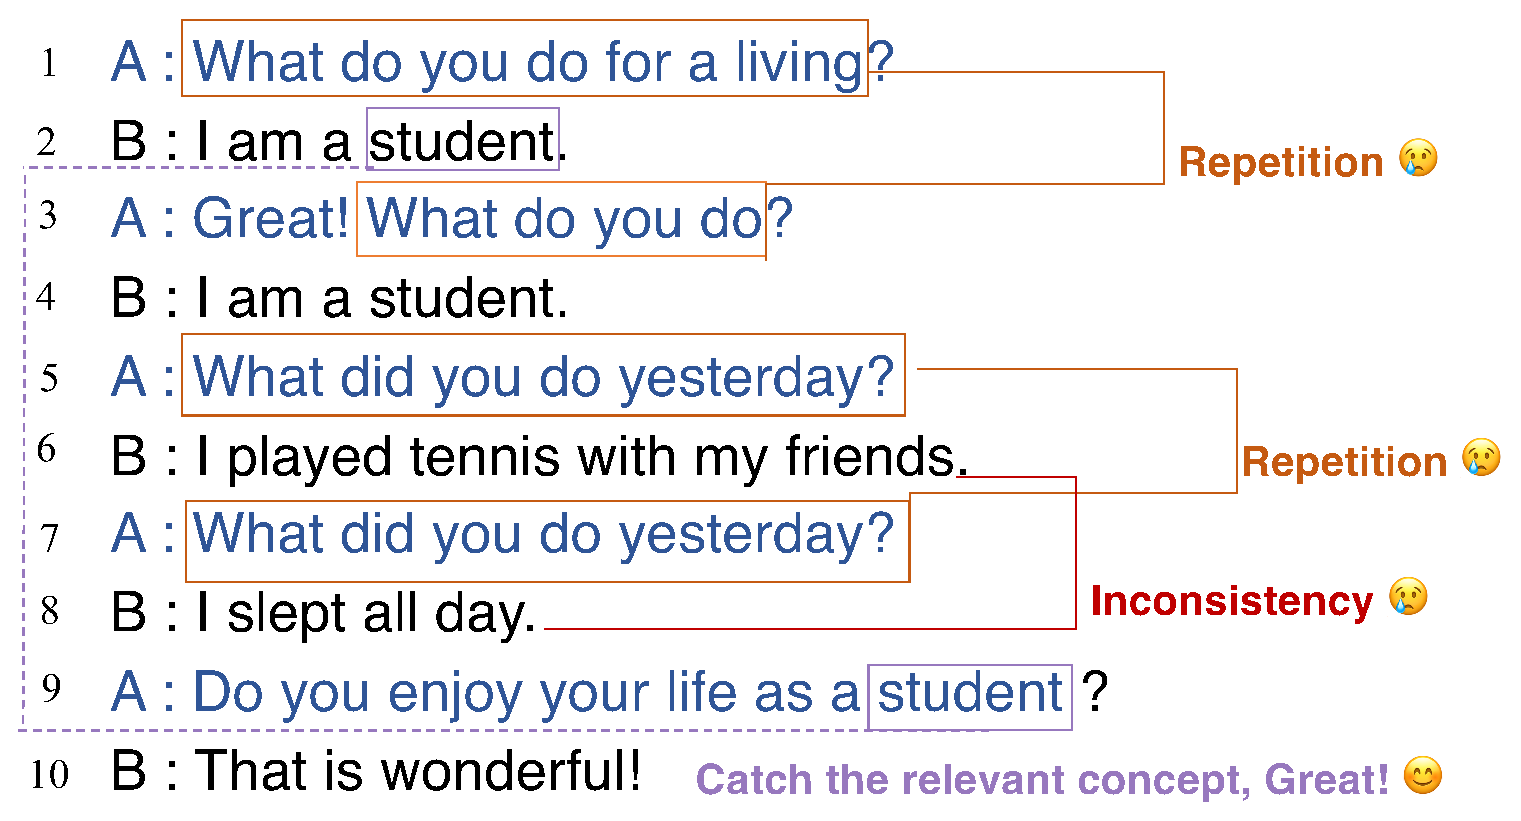
\includegraphics[width=0.95\columnwidth]{example2.eps}
        \caption{A chat snippet between two bots.}
        \label{fig:example}
\end{figure}

Fluency, Knowledge, Proactivity and Specificity are scored for each turn separately
and aggregated at the end of the conversation.
Detection for diversity, consistency and relevance are more involved and are explained
using \figref{fig:example}. 

As for diversity, at each turn $t$, we first check if there exists any repetitive question.  
We can easily find turn 3 and turn 7 repeated turn 1 and turn 5 
respectively. They will then be penalized one point for repetition. 
Repetition is not penalized if the previous turn is already 
marked as a repetitive question. For example, in \figref{fig:example}, 
although turn 4 is considered a repetition of turn 2,  
we are not going to penalize it as turn 3 is a repetitive question. 

The detection of inconsistency is always triggered after the detection of repeated questions. 
If the answers to the same questions are different, we will penalize the current turn, 
such as turn 8 in \figref{fig:example}.

We decide a repetition or an inconsistency by calculating the similarity of the two turns. 
We use a similarity function to complete the calculations, which we will 
discuss in \secref{sec:experiment}. The actual diversity and consistency scores
are the negation from the amount of repetition and inconsistency.

Relevance is assessed as a bonus to reward
a bot if it is able to memorize the important relevant concepts that have shown up 
before in the conversation. We sort the concepts that have shown up in 
chat history by their IDF scores. For example, in turn 9, $A$ 
mentions the concept word ``student'' presented by $B$ in turn 2. With this
turn, $A$ will win a bonus point.


The algorithms and notations for computing diviersty, consistency and relevance are included
in \tabref{tab:functions}, \algoref{algo:rep}, \algoref{algo:inconsist}, and \algoref{algo:bonus}. 

\begin{table}[th]
\centering
\small
\begin{tabular}{c|l}
%\hline
\toprule
\textbf{Notation} & \textbf{Description} \\ \midrule
$t$ & Current turn \\
$H(t)$  &  a list of history turns prior to $t$ \\
$Sim(x,y)$ & similarity between two turns $x$ and $y$ \\
$\sigma_r$ & Threshold for detecting repetition \\
$\sigma_c$ & Threshold for detecting consistency \\
$r$ & Weight for repetition \\
$c$ & Weight for inconsistency \\
$b$ & Weight for bonus \\
$d$ & Min distance between consecutive mentions \\
IDF list & List of lemma in chatlog sorted by IDF\\
$p$ & Percentage of important lemmas in IDF list\\
$R(t)$ &  Repetition penalty for turn $t$ \\
$C(t)$ &  Inconsistency penalty for turn $t$ \\ 
$B(t)$ &  Memory bonus for turn $t$ \\
$Rep(t)$ & A list of repeated turns for turn $t$ \\  
\bottomrule
\end{tabular}
\caption{
Functions and variables in algorithms.}
\label{tab:functions}
\end{table}

\begin{algorithm}[th]
\small
\caption{Scoring for Diversity}
\label{algo:rep}
\hspace*{0.02in} {\bf Input:}
 $t$, $H$, $Sim$, $\sigma_{r}$
; \hspace*{0.02in} {\bf Output: } 
 $R$;
\begin{algorithmic}[1]
\State //Starting to detect repetition
\For {$u$ in $H(t)$}
	\If {$Sim(t,u) \geq \sigma_{r}$}
		\State Add $u$ to $Rep(t)$
	\EndIf
\EndFor
    \If{$len(Rep(t))\geq 0$}
        \If{$t$ is a question and We can find a question in $Rep(t)$}
        \State $ R(t) \leftarrow  R(t) + 1$ 
        \Else
        \If {the previous turn of $t$ is not a repetitive question}
        \State $R(t)) \leftarrow R(t) + 1$ 
        \EndIf
        \EndIf
    \EndIf
\end{algorithmic}
\end{algorithm}


\begin{algorithm}[th]
\small
\caption{Scoring for Consistency}
\label{algo:inconsist}
\hspace*{0.02in} {\bf Input:}
$t$, $H$, $Sim$, $\sigma_{c}$
; \hspace*{0.02in} {\bf Output:  } 
 $C$;
\begin{algorithmic}[1]
\State // Inconsistency detection
 \If {previous turn of $p$ is a repetitive question} 
   \If{ the response $res$ to the question repeated by turn $p$ contradicts turn $i$ with $Sim(t, res) \leq \sigma_{c}$ }
    \State $C(t) \leftarrow C(t) + 1$
   \EndIf
  \EndIf
\end{algorithmic}
\end{algorithm}

\begin{algorithm}[th]
\small
\caption{Scoring for Relevance}
\label{algo:bonus}
\hspace*{0.02in} {\bf Input:}
$t$, $p$, $d$
; \hspace*{0.02in} {\bf Output:  } 
$B$;
\begin{algorithmic}[1]
\State // Assessing the ability of catching relevant concepts\\
$B(t) \leftarrow 0$
\For {all tokens $tk$ in current turn $t$}
 \If {$t$ - previous occurrence turn of $tk > d$ and $tk$ in the top $p\%$ of the IDF list of all tokens in the dialogue} 
   \State $B(t) \leftarrow 1$
  \EndIf
 \EndFor
\end{algorithmic}
\end{algorithm}

At the end of each game, each bot gets seven scores, one for each dimension.  
After pairwise comparison on individual dimension, a bot gains one point for win and zero point for a tie or lose.
The final score of each bot is determined by the sum of their individual scores.
%\KZ{Are these scores positive or negative? Comparable between bots?}

\subsubsection*{Match-level Scoring}
%\KZ{Use an equation to compute the final scores?}
One match which consists of two games, each started with a different bot, 
decides winning or losing between two bots.
For match-level scoring, we mimic the scoring rules of soccer tournament. 
For each match, $W$ points for the winner,  
$T$ points for a tie and 
$L$ points for the loser.
The value of $W$, $T$ and $L$ will be discussed in \secref{sec:ablation}. 

%\KZ{At the match level, we need to consider different starting context for the bots? I think we should present a few options for the reader and say that we are limited to these.}

\subsubsection*{Tournament-level Scoring}
%\KZ{Use an equation to compute the final scores?}
We count the points by simply summing up their scores gained in every match. Currently, several bots with the same final rank are tolerated. For future study, it's possible to mimic more detailed rules presented in sports match such as determine their ranking based on their win-loss relationship in the match between them.  
If they are still tied, we could propose an “overtime” for these two bots, one human judge may observe their performance and then make the decision of the game.


\subsection{Different Decoder Models}
Zheng et al. used relative complex variant of LSTM as the simple RE tagging
decoder. Evaluate the effectiveness of different alternatives, 
we compare Zheng's LSTM cell with two popular
RNN cells, namely normal LSTM and GRU on the basic RE tagging task.
To enable comparison with Zheng's results, we use order-first algorithm to
construct triples. \tabref{tab:decode} shows the results.

\begin{table}[th!]
  \begin{center}
  \small
  \caption{Results from Different Decoders}
  \label{tab:decode}
    \begin{tabular}{c|ccc}
      \hline
      \bf Models & \bf Prec. & \bf Rec. & \bf F1 \\
      \hline
      Zheng-LSTM  & \textbf{.615} & .414 & .495 \\
      LSTM   & .592 & .444 & \textbf{.507} \\
      GRU    & .579 & .438 & .499 \\
      \hline
    \end{tabular}
  \end{center}
\end{table}

Vanilla LSTM beats the rest by narrow margin in F1. 
We can conclude that Zheng's complex LSTM is not any better than the
basic LSTM, therefore in all other experiments, we adopt the vanilla
LSTM as our decoder.
%no much difference in F1 value between 4 LSTM cells. This conclusion is
%consistent with many work by others. However, the ability to balance precision
%and recall is really diffenrent. The difference between precision and recall
%values is beyond $0.20$, while this difference of any one of other 3 LSTM cell
%is limited in $0.15$. The precision value of Zheng is the highest and the recall
%is the lowest. Therefore,  we choose Pure-LSTM as our decoder in later experiments.


\subsection{Different Construction Algorithm}
In this experiment, we compare three different triple construction algorithms
in \tabref{tab:cons1}. $e_1$-first algorithm has a clear advantage
than $e_2$-first, which is in turn better than the default order-first.
This can be explained if we look at the accuracy of $e_1$ and $e_2$ in
the RE-tagging results in \tabref{tab:cons2}.
\begin{table}[th!]
  \small
  \begin{center}
  \caption{Different Construction Algorithms on Triple Accuracy}
  \label{tab:cons1}
    \begin{tabular}{c|ccc}
      \hline
      \bf Models & \bf Prec. & \bf Rec. & \bf F1 \\
      \hline
      $e_1$-first   &  \textbf{.631} & \textbf{.480} & \textbf{.545}  \\
      $e_2$-first   &  .605 & .450 & .516  \\
      Order-first  &  .592 & .444 & .507  \\
      \hline
    \end{tabular}
  \end{center}
\end{table}

\KZ{Add another algorithm that gives the nearest pairs.}
From \tabref{tab:cons2}, the accuracy for tagging $e_1$ is higher than
$e_2$ consistently. \KZ{Why is that?} As a result, the $e_1$-centric 
triple construction algorithm gives better overall accuracy than if we
use $e_2$ as the dominating entity. Order-first algorithm is worst because
it imposes a strict order of selecting entity pairs, which is more brittle
than other two algorithms. In the rest of this section, we will
use $e_1$-first as our triple construction algorithm.

\begin{table}[th!]
  \small
  \begin{center}
  \caption{RE Tagging Accuracy on the Entities}
  \label{tab:cons2}
    \begin{tabular}{ccc|ccc}
      \hline
       \multicolumn{3}{c|}{$e_1$} & \multicolumn{3}{c}{$e_2$} \\
      \hline
      	 Prec. & Rec. & F1 & Prec. & Rec. & F1 \\
      \hline
%        .650 & .606 & .627 & .616 & .603 & .609 \\
        .660 & .603 & .630 & .622 & .600 & .610 \\
%        .653 & .594 & .621 & .620 & .601 & {\bf .610} \\
      \hline
    \end{tabular}
  \end{center}
\end{table}



%As we can see from table 3, Order-First is worst, and Ele2-First is a little better
%than Order-First. Ele1-First is the best algorithm which achieve near $4$
%percent points than Order-First. The reason can be found in tabel 4 which show
%the preformance on signle element and element pair.
%
%The metrics on $e_1$ and elment2 is very near between these 3 experiments.
%Because the only different between these 3 experiments is the construction algorithm
%which do not take part in the training process. The ability to predict correct tag
%sequence should be near each other. The prediction of signle element has nothing
%to do with construction algorithm. By comparing the performance of $e_1$ and
%$e_2$, we can find the ability to predict correct $e_1$ is pretty high
%than $e_2$. The recall value of $e_1$ and $e_2$ is all most the same.
%But the precision values have a big difference. This means the model has predict
%more wrong $e_2$ than $e_1$. In other word, there is more correct $e_1$
%than $e_2$. Therefore, it is better to choose $e_1$ as the dominating
%entity rather than $e_2$. This is the reason why Ele1-Frist outperforms
%Ele2-First a lot. Order-First treats $e_1$ and $e_2$ in equal position
%which means this algorithm depends on the accuracy of both $e_1$ and
%$e_2$. In other words, the performance of Order-First is limited by the worse
%one of the two elements. This is the reason why Order-First is a little worse
%than Ele2-Frist.

\subsection{End-to-end RE Results}
%We have proved Pure-LSTM is more suitable for the decoder of EndRE module in 4
%kinds of LSTM cells. And Ele1-First algorithm is the best one to construct
%triple from relation tag sequence. We test the performance of our full
%multi-task model based on Pure-LSTM and Ele1-Frist algorithm. 
\tabref{tab:e2e} shows the accuracy of end-to-end relation triple extraction from
all baseline methods as well as our methods. Because our method enhances
Zheng's LSTM-LSTM-Bias (LLB) model, we name our method LLB+, which means
LLB plus RTD.

\begin{table}[th!]
  \small
  \begin{center}
    \begin{tabular}{cccc}
      \hline
      \bf Models & \bf Prec. & \bf Rec. & \bf F1 \\
      \hline
      FCM & .553 & .154 & .240 \\
      DS+logistic & .258 & .393 & .311 \\
      LINE & .335 & .329 & .332 \\
      \hline
      MultiR & .338 & .327 & .333 \\
      DS-Joint & .574 & .256 & .354 \\
      CoType & .423 & .511 & .463 \\
      \hline
      LSTM-CRF & \textbf{.693} & .310 & .428 \\
      LSTM-LSTM & .682 & .320 & .436 \\
      LSTM-LSTM-Bias & .615 & .414 & .495 \\
      \hline
      LLB+ & .623 & \textbf{.517} & \textbf{.565} \\
%      LLB+ (-NER) & .618 & .513 & .561 \\
      LLB+ (-RTD) & .618 & .498 & .552 \\
%      LLB+ (-NER-RTD) & .631 & .480 & .545 \\
      \hline
    \end{tabular}
  \end{center}
  \caption{End-to-end RE Results}
  \label{tab:e2e}
\end{table}

\begin{table*}[th!]
  \small
  \begin{center}
  \caption{Accuracy of Entity Tagging}
  \label{tab:entity}
    \begin{tabular}{c|ccc|ccc}
      \hline
      Entity & \multicolumn{3}{|c|}{E1} & \multicolumn{3}{|c}{E2} \\
      \hline
      	& Prec. & Rec. & F1 & Prec. & Rec. & F1 \\
      \hline
      LSTM-CRF & .596 & .325 & .420 & .605 & .325 & .423 \\
      LSTM-LSTM & .593 & .342 & .434 & .619 & .334 & .434 \\
      LSTM-LSTM-Bias & .590 & .479 & .529 & .597 & .451 & .514 \\
      \hline
      LLB+  & .628 & .657 & .642 & .594 & .647 & .619 \\
%      LLB+ (-NER) & .620 & .649 & .634 & .589 & .645 & .615 \\
      LLB+ (-RTD) & .623 & .661 & .641 & .592 & .647 & .618 \\
%      LLB+ (-NER-RTD) & .650 & .606 & .627 & .616 & .603 & .609 \\
      \hline
    \end{tabular}
  \end{center}
\end{table*}

Compared to the state-of-art model LSTM-LSTM-Bias, our method LLB+
logged 7\% substantial improvement on F1. This gain is primarily due to 
the advantage in recall, which is more than 10\%. 
%The precision values between LSTM-LSTM-Bias and MT-EndRE is not different
%too much, but MT-EndRE improve the recall value very much which achieves more
%than $10$ percent points gain. 
By looking at the accuracying of tagging $e_1$ and $e_2$ in \tabref{tab:entity}, 
we see that the recall of both $e_1$ and $e_2$ improve dramatically over 
LSTM-LSTM-Bias, while the precision remains relatively unchanged. 
This means our multi-task model predicts more entity pairs correctly
without lowering the precision.
%Therefore, our model can achieve remarkable gain in recall of relation triple.
%Finally, MT-EndRE can beat the state-of-the-art model a lot. Also our multi-task
%model is much better than all the pipeline and joint approches.

Further, to show the effect of the two auxiliary tasks in our model, we conduct
the ablation tests (shown in lowest section of \tabref{tab:e2e}). 
We find that the auxiliary task RTD is useful in boosting the basic RE model. 
%while RTD task provides more boost than NER.  
%LLB+(-NER-RTD) is the model without NER and RTD module 
%which is just the RE tagging module by itself. By comparing with full multi-task model
%MT-EndRE, without NER module the F1 value of triple will drop a little while
%without RTD module the F1 value will drop more. If getting rid of both NER and
%RTD, the performance will drop a lot. This means RTD module can provide more
%help to the EndRE by comparision with NER. There may be two reasons which cause
%RTD is more helpful than NER. 
This is because 
%i) NER is a relatively easy task, and previous research has shown
%accuracy above 0.92, so the basic RE tagging module itself can handle it
%rather well; ii) 
RC is a harder task but its relative, RTD, is able to  
provide global information of whole sentence which
complement the information obtained by the RE tagging alone. 
\KZ{Say a little more here?}

\subsection{Case Study}
To illustrate the effectiveness of our proposal, we present two cases
from the test set. The first sentence is used to show the effectiveness of our
joint model LLB+ by comparing with LLB. \{India, Contains, Bihar\} is the gold
triple. Both LLB+ and LLB mistake the number ``351'' as $e_2$ because
of the misleading context ``in''. Based on the tag of ``351'', LLB treat
``Bihar'' as the $e_2$ which is wrong. However, the LLB+ model 
predicts ``Bihar'' as $e_2$ which seems to conflict with the existing $e_2$ ``351''.
``India'' is predicted as $e_1$ correctly for two models. Eventually, 
LLB+ succeeds in constructing the correct triple. 
This is because LLB heavily relies on the local information (nearby entities) 
while LLB+ has a more global view.

The second sentence illustrates the difference between the triple construction
algorithms. In this case, all of the construction algorithms operates on the
same RE tag sequence. $e_x$-first re-constructs the correct triple \{Iowa,
Contains, Waverly\} while order-first does not. Because this tag sequence contain
several redundant $e_2$, the correct $e_2$ is the nearest to $e_1$ ``Iowa''.
However, order-first algorithm re-constructs the wrong triples \{Iowa,
Contains, Wartburg College\}. As for $e_2$-First, it only
predicts the two correct entities, it can only re-construct one triple which is
the correct one. \KZ{Find another example with the same tag sequence.}

\begin{table*}[th!]
  \small
  \begin{center}
  \caption{Two Examples in Case Study}
  \label{tab:case}
    \begin{tabular}{lp{12cm}}
      \hline
      Gold Standard 1& the death toll stood at 351 in Bihar[Contains-2-S] state , which is home to this village and many others sitting on some of the most vulnerable floodplains in India[Contains-1-S] . \\
      LLB+ & the death toll stood at 351[Contains-2-S] in Bihar[Contains-2-S] state , ... the most vulnerable floodplains in India[Contains-1-S] . \\
      LLB & the death toll stood at 351[Contains-2-S] in Bihar[Country-1-S] state , ...  the most vulnerable floodplains in India[Contains-1-S] . \\
      \hline
      Gold Standard 2 & Jean-Luc Portal , 51 , a wine consultant in Somers[Contains-2-S] who grew up in the tiny village of Alzonne[Contains-2-S] in southern France[Contains-1-S] , said he became obsessed with the game when he was 6 . \\
      LLB ($e_1$-First) & \{ France, Contains, Alzonne \} \\
      LLB ($e_2$-First) & \{ France, Contains, Somers \} \\
      LLB (Order-First) & \{ France, Contains, Somers \} \\
      \hline
    \end{tabular}
  \end{center}
\end{table*}







\section{Acknowledgement}
This work was partially supported by NSFC (Grant Nos. 61033002 and
61003218).

\bibliographystyle{abbrv}
\renewcommand{\baselinestretch}{0.90}
\bibliography{mobile}

% sigproc.bib is the name of the Bibliography in this case
% You must have a proper ".bib" file
%  and remember to run:
% latex bibtex latex latex
% to resolve all references
%
% ACM needs 'a single self-contained file'!
%
%APPENDICES are optional
%\balancecolumns
%\appendix
%Appendix A

\end{document}
